\chapter{Membranas e transporte de membrana}\label{ch:b1:membranes-transport}

Ponha uma hemácia em água pura e ela incha e estoura em menos de um
segundo; ponha-a em salmoura e ela murcha. Devolva-a ao plasma e ela
mantém a forma bicôncava por quatro meses, bombeando sódio para fora e
potássio para dentro em cada segundo desse tempo. A membrana que faz
isso tem cinco nanômetros de espessura --- uma película de lipídios com
duas moléculas de profundidade, entremeada de proteínas --- e é a
fronteira através da qual, no fim das contas, acontece cada troca do
\cref{ch:b1:organism-environment}. Este capítulo descreve a estrutura da
membrana, a física do que a atravessa sem ajuda, as proteínas que
transportam, bombeiam e canalizam o resto, o potencial elétrico que esse
tráfego produz, e as vesículas que carregam o que nenhuma proteína
carrega.

\section{O mosaico fluido}

\begin{definition}[A membrana plasmática]\label{def:b1:membranes-transport:membrane}
A \emph{membrana plasmática}\index{membrana plasmática} --- e toda
membrana da \omterm{def:b1:cell-unit-of-life:cell}{célula} --- é uma
\emph{bicamada lipídica}\index{bicamada lipídica} de cerca de
\qty{5}{nm} de espessura: duas lâminas de fosfolipídios
(\cref{ch:b1:lipids}) com as caudas hidrofóbicas voltadas umas para as
outras e as cabeças polares voltadas para os dois lados aquosos, com
colesterol entre as caudas, e
\emph{proteínas de membrana}\index{proteína de membrana} embutidas nela
ou presas a ela. No modelo do
\emph{mosaico fluido}\index{modelo do mosaico fluido} (Singer e
Nicolson, 1972) a bicamada é um fluido bidimensional em que lipídios e
proteínas se difundem lateralmente, e as proteínas são um mosaico de
unidades independentes, e não um revestimento contínuo. As duas faces
diferem: os açúcares presos a lipídios e proteínas ficam voltados apenas
para fora (o \emph{glicocálice}), e alguns fosfolipídios ficam confinados
a um só folheto.
\end{definition}

\begin{omfigure}
\begin{tikzpicture}[font=\footnotesize, line cap=round]
  % bilayer: heads as circles, tails as lines
  \foreach \i in {0,...,21} {
    \pgfmathsetmacro{\x}{0.42*\i}
    \fill[omDef!60] (\x,1.35) circle (0.16);
    \draw[omDef!70!black, thick] (\x-0.07,1.2) -- (\x-0.07,0.55) (\x+0.07,1.2) -- (\x+0.07,0.55);
    \fill[omDef!60] (\x,-0.35) circle (0.16);
    \draw[omDef!70!black, thick] (\x-0.07,-0.2) -- (\x-0.07,0.45) (\x+0.07,-0.2) -- (\x+0.07,0.45);
  }
  % cholesterol
  \foreach \x in {1.9,6.1,8.2} { \draw[omProp, very thick] (\x,1.1) -- (\x,0.6); \fill[omProp] (\x,1.15) circle (0.08); }
  % integral protein spanning (channel)
  \draw[thick, omThm!80!black, fill=omThm!30, rounded corners=3pt] (3.0,-0.7) rectangle (3.55,1.7);
  \draw[thick, omThm!80!black, fill=omThm!30, rounded corners=3pt] (3.85,-0.7) rectangle (4.4,1.7);
  \fill[white] (3.55,-0.6) rectangle (3.85,1.6);
  % integral protein (carrier)
  \draw[thick, omThm!80!black, fill=omThm!30, rounded corners=5pt] (6.8,-0.75) rectangle (7.7,1.75);
  % peripheral protein
  \draw[thick, omExo!80!black, fill=omExo!30] (5.3,1.75) ellipse (0.5 and 0.28);
  % glycocalyx sugar chains on outer face
  \foreach \x in {0.5,1.3,2.5,4.15,7.25,8.4} { \draw[omProp!80!black, thick] (\x,1.5) .. controls (\x+0.15,1.85) and (\x-0.15,2.1) .. (\x+0.1,2.4); \fill[omProp!70] (\x+0.1,2.45) circle (0.07); }
  % labels
  \node[anchor=east] at (-0.3,1.35) {cabeças polares};
  \node[anchor=east] at (-0.3,0.5) {caudas hidrofóbicas};
  \node[anchor=east] at (-0.3,-0.35) {cabeças polares};
  \node[anchor=west, align=left] at (9.2,2.2) {cadeias de açúcar:\\ só do lado de fora};
  \node[anchor=west, align=left] at (9.2,0.5) {\qty{5}{nm}};
  \node[anchor=north] at (3.7,-0.95) {proteína de canal};
  \node[anchor=north, align=center] at (7.25,-0.95) {proteína\\ transportadora};
  \node[anchor=south] at (5.3,2.6) {proteína periférica};
  \node[anchor=north, omProp] at (1.5,-1.0) {colesterol};
  \node[anchor=south east, gray] at (-0.3,2.4) {exterior};
  \node[anchor=north east, gray] at (-0.3,-0.95) {citosol};
  \draw[<->, gray] (9.05,1.35+0.16) -- (9.05,-0.35-0.16);
\end{tikzpicture}

{\small O \omterm{def:b1:membranes-transport:membrane}{mosaico fluido}. Dois folhetos de fosfolipídios, com as caudas
para dentro e colesterol entre elas; proteínas \omterm{def:b1:membranes-transport:proteins}{integrais} atravessando a
bicamada (um \omterm{def:b1:membranes-transport:transporters}{canal} com o poro dele, um transportador), uma proteína
periférica numa das faces, e cadeias de açúcar somente na face externa.}
\end{omfigure}

\begin{omfigure}
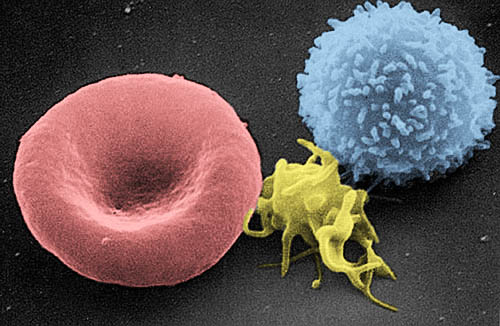
\includegraphics[width=0.4\linewidth]{images/book3/red-cells-nci.jpg}

{\small Uma hemácia, uma plaqueta e um linfócito ao \omterm{prop:b1:cell-unit-of-life:microscopes}{microscópio
eletrônico} de varredura (imagem colorizada). A forma bicôncava da
hemácia é mantida por uma malha de proteínas sob a membrana dela; ela
sobrevive a quatro meses de compressão em capilares mais estreitos que
ela própria. Imagem: National Cancer Institute, domínio público.}
\end{omfigure}

\begin{proposition}[As membranas são bicamadas e são fluidas]\label{prop:b1:membranes-transport:evidence}
A \omterm{def:b1:membranes-transport:membrane}{membrana plasmática} tem exatamente duas moléculas de lipídio de
espessura, e os componentes dela se movem dentro do plano dela.
\end{proposition}
\begin{proof}[Evidências]
Gorter e Grendel (1925) extraíram os lipídios de um número conhecido de
hemácias e os espalharam como monocamada sobre água: a área era o dobro
da superfície total das \omterm{def:b1:cell-unit-of-life:cell}{células}, e portanto a membrana é uma bicamada. A
microscopia eletrônica mostra toda membrana como duas linhas escuras (as
cabeças coradas) em torno de um núcleo pálido (as caudas), com
\qty{5}{nm} no total. Frye e Edidin (1970) fundiram uma \omterm{def:b1:cell-unit-of-life:cell}{célula} de
camundongo com uma \omterm{def:b1:cell-unit-of-life:cell}{célula} humana cujas proteínas de superfície tinham
sido marcadas com corantes de duas cores: depois de quarenta minutos a
\qty{37}{\celsius} as duas cores estavam completamente misturadas por
toda a \omterm{def:b1:cell-unit-of-life:cell}{célula} híbrida, e não a \qty{4}{\celsius}, em que o lipídio está
quase sólido. Branquear com um laser uma mancha de uma \omterm{def:b1:membranes-transport:membrane}{proteína de
membrana} fluorescente e observar a fluorescência voltar à medida que
moléculas não branqueadas se difundem para lá (FRAP) mede a difusão
lateral: $\qty{1}{\micro m^2}$ em alguns segundos para os lipídios, mais
lenta para as proteínas, e nula para as proteínas ancoradas ao
\omterm{def:b1:eukaryotic-cell:cytoskeleton}{citoesqueleto}.
\end{proof}

\begin{definition}[Proteínas de membrana]\label{def:b1:membranes-transport:proteins}
As proteínas \emph{integrais}\index{proteína integral} de membrana
atravessam a bicamada com uma ou mais hélices hidrofóbicas e só podem
ser extraídas com detergentes; as proteínas \emph{periféricas} ficam
ligadas a uma das faces. Por função: os \emph{transportadores} (\omterm{def:b1:membranes-transport:transporters}{canais},
carreadores, bombas), os \emph{receptores}, que ligam um sinal do lado
de fora e agem do lado de dentro, as \emph{enzimas}, as
\emph{âncoras}, que ligam o \omterm{def:b1:eukaryotic-cell:cytoskeleton}{citoesqueleto} à \omterm{def:b1:body-plans-tissues:connective}{matriz extracelular}, e as
proteínas de \emph{reconhecimento}, que carregam os açúcares pelos quais
as \omterm{def:b1:cell-unit-of-life:cell}{células} se identificam umas às outras. As proteínas são metade da
massa de uma membrana típica e quase toda a função dela.
\end{definition}

\section{Atravessar a membrana sem ajuda}

\begin{proposition}[Permeabilidade da bicamada]\label{prop:b1:membranes-transport:permeability}
\index{permeabilidade}
Uma \omterm{def:b1:membranes-transport:membrane}{bicamada lipídica} pura é livremente permeável a moléculas apolares
pequenas ($\mathrm{O_2}$, $\mathrm{CO_2}$, $\mathrm{N_2}$, esteroides),
razoavelmente permeável a moléculas polares pequenas e sem carga (água,
ureia, etanol), pouco permeável a moléculas polares maiores (glicose,
aminoácidos), e praticamente impermeável a íons ($\mathrm{Na^+}$,
$\mathrm{K^+}$, $\mathrm{Cl^-}$, $\mathrm{H^+}$) e a macromoléculas. A
permeabilidade abrange doze ordens de grandeza, de $\qty{e-2}{cm/s}$
para a água a $\qty{e-14}{cm/s}$ para o $\mathrm{Na^+}$: um núcleo
hidrofóbico de \qty{3}{nm} de espessura deixa passar o que se dissolve
em óleo e barra o que carrega uma carga.
\end{proposition}

\begin{theorem}[Lei de Fick para a difusão]\label{thm:b1:membranes-transport:fick}
\index{lei de Fick}\index{difusão}
O fluxo líquido $J$ de um soluto através de uma membrana de área $S$
(em mols por segundo) é proporcional à diferença de concentração:
\[
J = P\,S\,(c_{\text{ext}} - c_{\text{int}}),
\]
em que o \emph{coeficiente de permeabilidade} $P$ (em \unit{m/s}) reúne
o coeficiente de difusão do soluto na membrana, a solubilidade dele no
lipídio e a espessura da membrana ($P = DK/\ell$). A difusão não precisa
de energia e corre sempre a favor do gradiente; ela é
\emph{transporte passivo}\index{transporte passivo}.
\end{theorem}
\begin{proof}
Dentro da membrana o soluto se difunde ao longo de um perfil linear de
concentração, de $Kc_{\text{ext}}$ a $Kc_{\text{int}}$ ($K$ é o
coeficiente de partição entre lipídio e água); a primeira \omterm{thm:b1:membranes-transport:fick}{lei de Fick} no
meio, $J/S = -D\,\dd c/\dd x$, dá $J/S = DK(c_{\text{ext}} -
c_{\text{int}})/\ell$.
\end{proof}

\begin{definition}[Osmose, potencial hídrico]\label{def:b1:membranes-transport:osmosis}
A \emph{osmose}\index{osmose} é a difusão líquida de água através de uma
membrana que deixa passar a água mas não os solutos, da solução em que a
água está mais concentrada (menos solutos) para aquela em que ela está
menos. Ela é descrita pelo
\emph{potencial hídrico}\index{potencial hídrico} $\Psi$, o potencial
químico da água expresso como pressão, nulo para água pura à pressão
atmosférica:
\[
\Psi = \Psi_s + \Psi_p, \qquad \Psi_s = -RTc_s ,
\]
em que $\Psi_s$, o
\emph{potencial osmótico}\index{potencial osmótico}, cai com a
concentração total de solutos $c_s$ (em osmoles por litro, a lei de van
't Hoff), e $\Psi_p$, o
\emph{potencial de pressão}\index{potencial de pressão}, é a pressão
hidrostática acima da atmosférica. A água se move do $\Psi$ maior para o
menor. A \qty{25}{\celsius}, $RT = \qty{2.48}{MPa.L/mol}$: uma solução de
\qty{0.3}{osmol/L} tem $\Psi_s = \qty{-0.74}{MPa}$. Uma solução é
\emph{isotônica}\index{isotônica} em relação a uma \omterm{def:b1:cell-unit-of-life:cell}{célula} quando não há
fluxo líquido de água, \emph{hipotônica} quando entra água,
\emph{hipertônica} quando ela sai.
\end{definition}

\begin{omfigure}
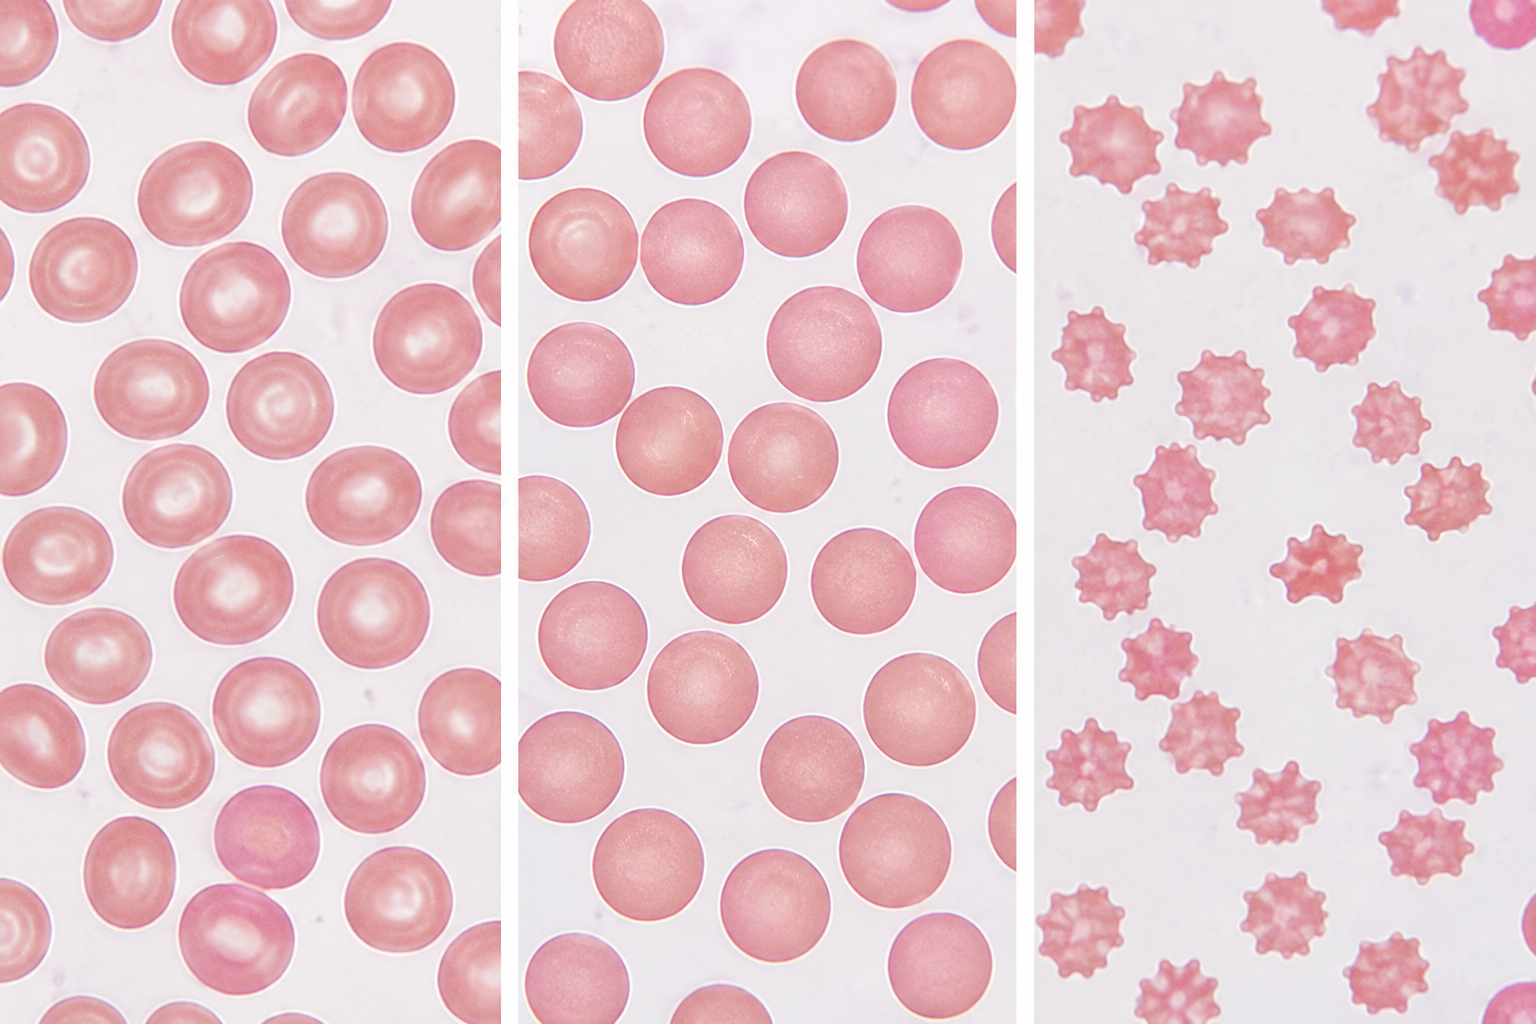
\includegraphics[width=0.78\linewidth]{images/book3/ai/b3-07-red-cells-osmosis.png}

{\small Hemácias numa solução \omterm{def:b1:membranes-transport:osmosis}{isotônica} (discos bicôncavos), numa
solução hipotônica (inchadas até virarem esferas, prestes a estourar) e
numa hipertônica (murchas e crenadas). A água segue o potencial dela; a
\omterm{def:b1:cell-unit-of-life:cell}{célula} não tem parede para resistir.}
\end{omfigure}

\begin{omfigure}
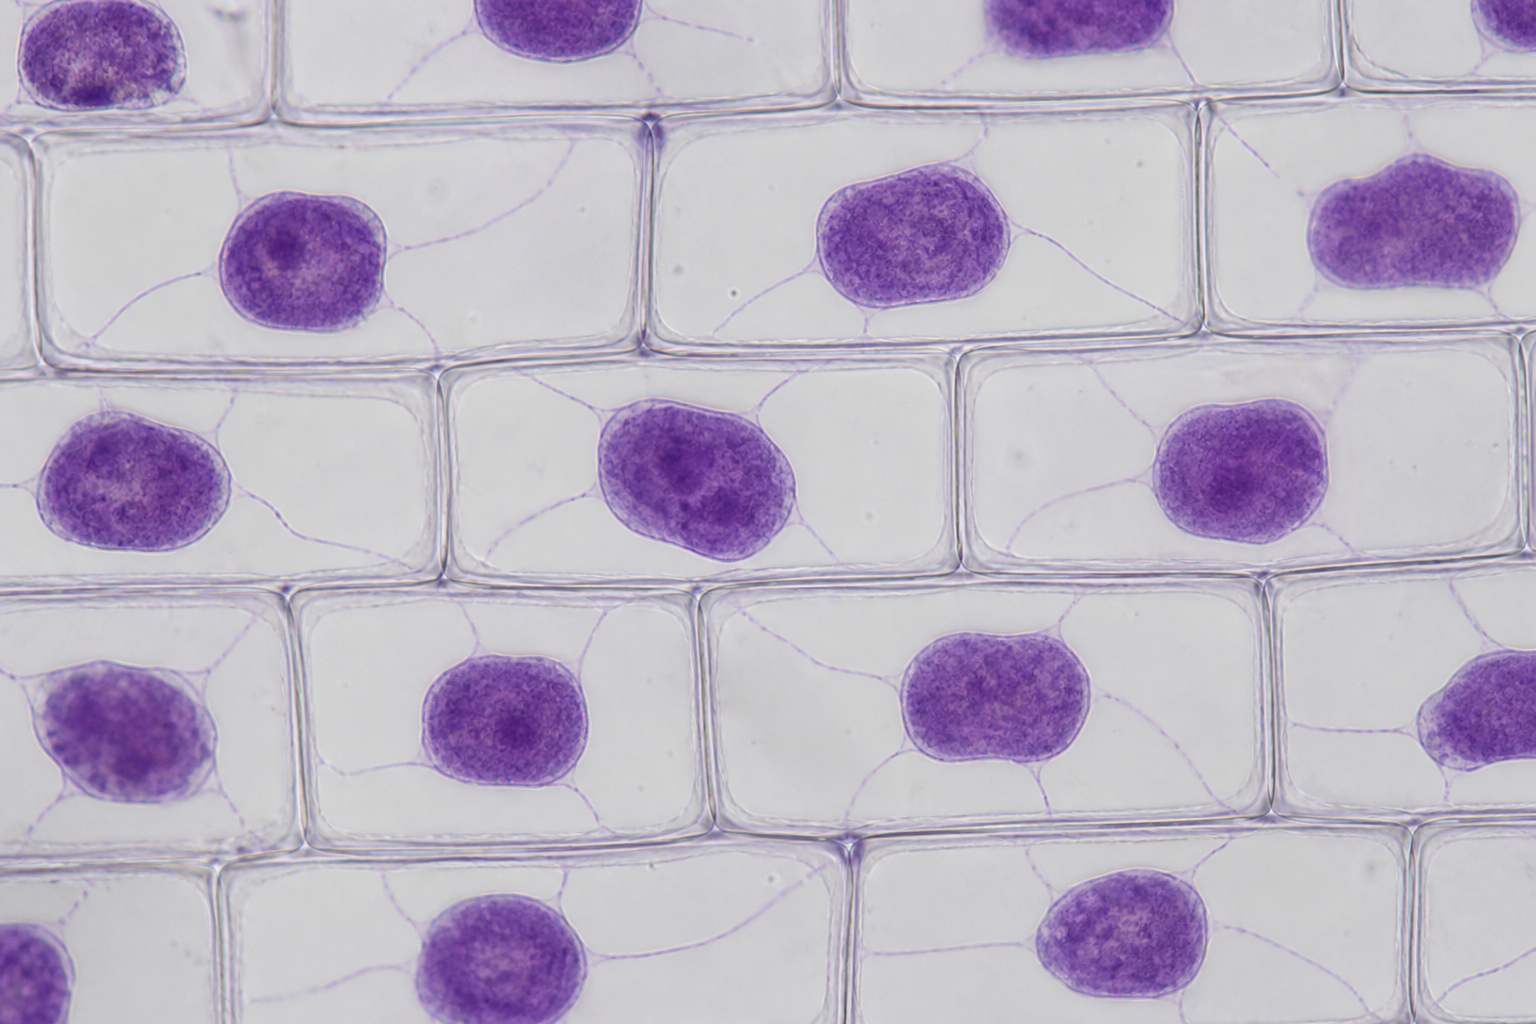
\includegraphics[width=0.6\linewidth]{images/book3/ai/b3-07-plasmolysis.png}

{\small Plasmólise: epiderme de cebola numa solução salina forte. O
protoplasto de cada \omterm{def:b1:cell-unit-of-life:cell}{célula} perdeu água e se afastou da parede rígida,
que conserva a forma dela. Em água o protoplasto voltaria a inchar
contra a parede e pararia, túrgido.}
\end{omfigure}

\begin{example}[Uma hemácia em três soluções]\label{ex:b1:membranes-transport:redcell}
O plasma é de \qty{0.3}{osmol/L}: $\Psi_s = \qty{-0.74}{MPa}$ dos dois
lados, sem fluxo líquido. Em água pura ($\Psi = 0$) a \omterm{def:b1:cell-unit-of-life:cell}{célula}, a
\qty{-0.74}{MPa} por dentro, capta água até que a membrana dela, que só
consegue esticar alguns por cento, se rompa. Em sal a \qty{0.6}{osmol/L}
ela perde água até que o interior fique igualmente concentrado, com
metade do volume. Uma \omterm{def:b1:cell-unit-of-life:cell}{célula} vegetal em água pura não estoura: à medida
que a água entra, a parede é esticada e $\Psi_p$ sobe até que
$\Psi_p = -\Psi_s$, o \omterm{def:b1:membranes-transport:osmosis}{potencial hídrico} interno seja nulo e o fluxo pare,
com a \omterm{def:b1:cell-unit-of-life:cell}{célula} túrgida a \qty{0.74}{MPa}.
\end{example}

\begin{method}[Fazer as contas do potencial hídrico]\label{met:b1:membranes-transport:psi}
\begin{enumerate}
  \item Converta cada concentração de soluto em osmoles (um sal que se
        dissocia em dois íons conta duas vezes) e calcule $\Psi_s =
        -RTc_s$.
  \item Acrescente o termo de pressão: $\Psi_p = 0$ para uma solução num
        recipiente aberto ou para uma \omterm{def:b1:cell-unit-of-life:cell}{célula} animal, positivo para uma
        \omterm{def:b1:cell-unit-of-life:cell}{célula} vegetal túrgida, negativo para água sob tensão num vaso
        de \omterm{def:b1:flowering-plant-organization:tissues}{xilema}.
  \item A água flui para o $\Psi$ menor. O equilíbrio é atingido quando
        os dois $\Psi$ se igualam: por diluição do conteúdo da \omterm{def:b1:cell-unit-of-life:cell}{célula}
        (\omterm{def:b1:cell-unit-of-life:cell}{célula} animal) ou por elevação da pressão (\omterm{def:b1:cell-unit-of-life:cell}{célula} vegetal).
  \item Leia o sinal do resultado como o sentido do fluxo, e o tamanho
        dele como a força motriz; a velocidade do fluxo também depende
        da permeabilidade da membrana à água, elevada cem vezes pelos
        \omterm{def:b1:membranes-transport:transporters}{canais} de \omterm{def:b1:membranes-transport:transporters}{aquaporina}.
\end{enumerate}
\end{method}

\section{Proteínas de transporte}

\begin{definition}[Canais, carreadores, bombas]\label{def:b1:membranes-transport:transporters}
Os \emph{canais}\index{canal} são proteínas \omterm{def:b1:membranes-transport:proteins}{integrais} com um poro cheio
de água pelo qual um íon ou uma molécula pequena específica se difunde a
favor do gradiente dele, a até $10^8$ por segundo; muitos têm
\emph{comporta}, abrindo-se em resposta a uma voltagem, a um ligante ou
a uma força mecânica. As \emph{aquaporinas}\index{aquaporina} são canais
de água. Os \emph{carreadores}\index{carreador} ligam o soluto deles em
uma das faces, mudam de conformação e o liberam na outra, no máximo mil
vezes por segundo; o transportador de glicose da hemácia é um deles.
Canais e carreadores que trabalham a favor de um gradiente realizam
\emph{difusão facilitada}\index{difusão facilitada}, passiva mas
seletiva e saturável. As \emph{bombas}\index{bomba} são carreadores que
acoplam o transporte de um soluto contra o gradiente dele à hidrólise de
ATP: o \emph{transporte ativo primário}\index{transporte ativo}. A
\emph{bomba de sódio e potássio}\index{bomba de sódio e potássio} das
\omterm{def:b1:cell-unit-of-life:cell}{células} animais exporta três $\mathrm{Na^+}$ e importa dois
$\mathrm{K^+}$ por ATP; a \emph{bomba de prótons} das membranas
vegetais, fúngicas e bacterianas exporta $\mathrm{H^+}$.
\end{definition}

\begin{omfigure}
\begin{tikzpicture}[font=\footnotesize, >=Stealth, line cap=round]
  % membrane band
  \fill[omDef!15] (0,0) rectangle (13.1,1.2);
  \draw[omDef!60!black] (0,0) -- (13.1,0) (0,1.2) -- (13.1,1.2);
  \node[anchor=east, gray, align=right] at (-0.15,1.5) {exterior\\ (muito $\mathrm{Na^+}$,\\ pouco $\mathrm{K^+}$)};
  \node[anchor=east, gray, align=right] at (-0.15,-0.3) {citosol\\ (pouco $\mathrm{Na^+}$,\\ muito $\mathrm{K^+}$)};
  % simple diffusion
  \draw[->, thick, omProp] (1.0,2.0) -- (1.0,-0.8);
  \node[anchor=south, align=center] at (1.0,2.1) {difusão simples\\ $\mathrm{O_2}$, $\mathrm{CO_2}$};
  % channel
  \draw[thick, omThm!80!black, fill=omThm!30, rounded corners=2pt] (2.6,-0.2) rectangle (3.0,1.4);
  \draw[thick, omThm!80!black, fill=omThm!30, rounded corners=2pt] (3.3,-0.2) rectangle (3.7,1.4);
  \draw[->, thick, omProp] (3.15,2.0) -- (3.15,-0.8);
  \node[anchor=south, align=center] at (3.15,2.1) {canal\\ $\mathrm{K^+}$, água};
  % carrier (facilitated)
  \draw[thick, omThm!80!black, fill=omThm!30, rounded corners=5pt] (5.0,-0.3) rectangle (6.0,1.5);
  \draw[->, thick, omProp] (5.5,2.0) -- (5.5,1.55);
  \draw[->, thick, omProp] (5.5,-0.35) -- (5.5,-0.8);
  \node[anchor=south, align=center] at (5.5,2.1) {carreador\\ glicose};
  \node[align=center, font=\scriptsize] at (5.5,0.6) {liga,\\ vira};
  % pump
  \draw[thick, omExo!80!black, fill=omExo!30, rounded corners=5pt] (7.5,-0.3) rectangle (8.7,1.5);
  \draw[->, very thick, omExo!80!black] (7.8,-0.8) -- (7.8,2.0);
  \draw[->, very thick, omExo!80!black] (8.4,2.0) -- (8.4,-0.8);
  \node[anchor=south, align=center] at (8.1,2.1) {bomba\\ $3\,\mathrm{Na^+}$ para fora, $2\,\mathrm{K^+}$ para dentro};
  \node[anchor=north, align=center, font=\scriptsize] at (8.1,-0.85) {ATP $\to$ ADP};
  % secondary active (symport)
  \draw[thick, omThm!80!black, fill=omThm!30, rounded corners=5pt] (11.0,-0.3) rectangle (12.2,1.5);
  \draw[->, very thick, omProp] (11.3,2.0) -- (11.3,-0.8);
  \draw[->, very thick, omExo!80!black] (11.9,2.0) -- (11.9,-0.8);
  \node[anchor=south, align=center] at (11.6,2.1) {simporte\\ $\mathrm{Na^+}$ desce,\\ glicose sobe};
  \node[anchor=north, align=center, font=\scriptsize] at (11.6,-0.85) {ativo secundário};
  \node[anchor=north west, align=left, gray, font=\scriptsize] at (0,-1.5) {setas laranja: a favor do gradiente (passivo);\\ setas verdes: contra ele (ativo)};
\end{tikzpicture}

{\small Cinco maneiras de atravessar. Difusão simples pelo lipídio; um
\omterm{def:b1:membranes-transport:transporters}{canal} e um carreador (\omterm{def:b1:membranes-transport:transporters}{difusão facilitada}, a favor do gradiente); a \omterm{def:b1:membranes-transport:transporters}{bomba
de sódio e potássio} (\omterm{def:b1:membranes-transport:transporters}{transporte ativo primário}, pago em ATP); e um
\omterm{prop:b1:membranes-transport:secondary}{simportador} que usa o gradiente de sódio construído pela bomba para
arrastar a glicose para cima (\omterm{prop:b1:membranes-transport:secondary}{transporte ativo secundário}).}
\end{omfigure}

\begin{proposition}[Transporte ativo secundário]\label{prop:b1:membranes-transport:secondary}
\index{transporte ativo secundário}
Um gradiente construído por uma bomba é um estoque de energia que outros
carreadores gastam: um \emph{simportador}\index{simportador} leva um
soluto para cima acoplando-o a um íon que desce no mesmo sentido (o
transportador de sódio e glicose do intestino e do rim; o transportador
de prótons e sacarose do floema), e um
\emph{antiportador}\index{antiportador} o acopla a um íon que se move no
sentido oposto (o trocador de sódio e cálcio). Nas \omterm{def:b1:cell-unit-of-life:cell}{células} animais a
moeda é o gradiente de $\mathrm{Na^+}$; nas plantas, nos fungos e nas
bactérias, o gradiente de $\mathrm{H^+}$.
\end{proposition}

\begin{example}[A cinética revela o mecanismo]\label{ex:b1:membranes-transport:kinetics}
O fluxo de glicose para dentro de uma hemácia sobe com a concentração
externa e depois se estabiliza num máximo, como o de uma enzima
(\cref{ch:b1:enzymes}): um carreador, saturável, com um $K_m$ de cerca
de \qty{1.5}{mmol/L}; um açúcar parecido, a manose, compete por ele. O
fluxo de ureia sobe proporcionalmente à concentração dela, sem limite:
difusão simples. O fluxo de glicose para dentro de uma \omterm{def:b1:cell-unit-of-life:cell}{célula} intestinal
para quando o sódio é retirado do lúmen, ou quando a bomba é envenenada
com ouabaína: \omterm{prop:b1:membranes-transport:secondary}{transporte ativo secundário}.
\end{example}

\section{O potencial de membrana}

\begin{definition}[Potencial de membrana]\label{def:b1:membranes-transport:potential}
Toda \omterm{def:b1:cell-unit-of-life:cell}{célula} viva mantém uma diferença de potencial elétrico através da
\omterm{def:b1:membranes-transport:membrane}{membrana plasmática} dela, o
\emph{potencial de membrana}\index{potencial de membrana}
$V_m = V_{\text{int}} - V_{\text{ext}}$, negativo por dentro:
\qty{-70}{mV} num \omterm{def:b1:body-plans-tissues:nervous}{neurônio}, \qty{-90}{mV} numa fibra muscular,
\qty{-120}{mV} ou mais numa \omterm{def:b1:cell-unit-of-life:cell}{célula} vegetal. Ele surge porque a membrana
é seletivamente permeável a íons cujas concentrações diferem dos dois
lados dela.
\end{definition}

\begin{theorem}[A equação de Nernst]\label{thm:b1:membranes-transport:nernst}
\index{equação de Nernst}\index{potencial de equilíbrio}
Um íon de carga $z$ nas concentrações $c_{\text{ext}}$ e
$c_{\text{int}}$ está em equilíbrio através da membrana --- sem fluxo
líquido, ainda que a membrana seja permeável a ele --- quando o
potencial iguala o \emph{\omterm{thm:b1:membranes-transport:nernst}{potencial de equilíbrio}} dele
\[
E_{\text{íon}} = \frac{RT}{zF}\,\ln\frac{c_{\text{ext}}}{c_{\text{int}}}
= \frac{\qty{61.5}{mV}}{z}\,\log_{10}\frac{c_{\text{ext}}}{c_{\text{int}}}
\quad (\qty{37}{\celsius}).
\]
Para o $\mathrm{K^+}$ a \qty{5}{mmol/L} fora e \qty{140}{mmol/L}
dentro, $E_K = 61.5\log(5/140) = \qty{-89}{mV}$; para o $\mathrm{Na^+}$ a
\qty{145}{} fora e \qty{12}{} dentro, $E_{Na} = \qty{+67}{mV}$.
\end{theorem}
\begin{proof}
Levar um mol do íon de fora para dentro muda a energia livre pela soma
de um termo de concentração e um termo elétrico:
\[
\Delta G = RT\ln\frac{c_{\text{int}}}{c_{\text{ext}}} + zFV_m .
\]
No equilíbrio $\Delta G = 0$, o que dá $V_m = (RT/zF)\ln(c_{\text{ext}}/c_{\text{int}})$.
Passar a logaritmos de base dez e substituir $R = \qty{8.314}{J.mol^{-1}.K^{-1}}$,
$T = \qty{310}{K}$ e $F = \qty{96485}{C/mol}$ dá a forma numérica.
\end{proof}

\begin{proposition}[Origem do potencial de repouso]\label{prop:b1:membranes-transport:resting}
A membrana em repouso é muito mais permeável ao $\mathrm{K^+}$ (por
\omterm{def:b1:membranes-transport:transporters}{canais} de potássio abertos) que ao $\mathrm{Na^+}$; o $\mathrm{K^+}$
vaza para fora a favor do gradiente de concentração dele, deixando o
interior negativo, até que a atração elétrica de volta quase equilibre o
vazamento. O potencial de repouso fica, portanto, perto de $E_K$,
puxado um pouco em direção a $E_{Na}$ pelo pequeno vazamento de sódio (a
equação de Goldman pondera o termo de Nernst de cada íon pela
permeabilidade dele). A bomba sustenta os gradientes que os vazamentos
dissipariam; ela também contribui com alguns milivolts diretamente, já
que move três cargas para fora a cada duas para dentro.
\end{proposition}
\begin{proof}[Evidências]
Num axônio de lula o potencial de repouso segue $E_K$ quando o potássio
externo é variado numa faixa ampla (uma reta de inclinação
\qty{58}{mV} por década em concentrações altas), e se afasta dele em
concentrações baixas exatamente como uma pequena permeabilidade ao sódio
prevê. Bloquear a bomba com ouabaína deixa o potencial quase inalterado
por minutos, e depois o deixa decair ao longo de horas à medida que os
gradientes se esgotam: o potencial é um potencial de difusão, e a bomba
é o sustentáculo dele a longo prazo.
\end{proof}

\begin{omfigure}
\begin{tikzpicture}
\begin{semilogxaxis}[
  width=0.86\linewidth, height=6.2cm,
  axis x line=bottom, axis y line=left,
  xmin=0.8, xmax=200, ymin=-135, ymax=10,
  xlabel={$\mathrm{K^+}$ externo (\unit{mmol/L})}, ylabel={potencial de membrana (\unit{mV})},
  xlabel style={font=\small, at={(axis description cs:0.5,-0.12)}, anchor=north},
  ylabel style={font=\small},
  tick label style={font=\small}, xtick={1,10,100}, log ticks with fixed point, ytick={-120,-100,-80,-60,-40,-20,0},
  legend style={font=\small, at={(0.03,0.97)}, anchor=north west, draw=none},
  clip=false,
]
\addplot[thick, dashed, omDef, domain=0.8:200, samples=40] {58*log10(x/140)};
\addlegendentry{Nernst $E_K$ (inclinação de \qty{58}{mV} por década)}
\addplot[very thick, omThm, domain=0.8:200, samples=60] {58*log10((x+0.01*145)/(140+0.01*12))};
\addlegendentry{medido: $\mathrm{K^+}$ mais um pequeno vazamento de $\mathrm{Na^+}$}
\draw[dashed, gray] (axis cs:5,-135) -- (axis cs:5,-82);
\node[font=\scriptsize, anchor=west] at (axis cs:5.5,-120) {\qty{5}{mmol/L} fisiológicos};
\end{semilogxaxis}
\end{tikzpicture}

{\small Potencial de repouso em função do potássio externo. Com potássio
alto a membrana se comporta como um eletrodo de potássio e segue a reta
de Nernst; com potássio baixo o pequeno vazamento de sódio o puxa acima
de $E_K$.}
\end{omfigure}

\begin{example}[Para onde vai a energia da bomba]\label{ex:b1:membranes-transport:pumpcost}
Bombear um $\mathrm{Na^+}$ para fora, contra a passagem de \qty{12}{} a
\qty{145}{mmol/L} e contra \qty{-70}{mV}, custa
$RT\ln(145/12) + F\times 0.070 = 6.4 + 6.8 =
\qty{13.2}{kJ/mol}$; três deles, \qty{40}{kJ}, mais dois
$\mathrm{K^+}$ para dentro a $RT\ln(140/5) - F\times 0.070 = 8.6 - 6.8 =
\qty{1.8}{kJ/mol}$ cada: \qty{43}{kJ} por ciclo contra os \qty{50}{kJ}
de um ATP nas condições celulares. A bomba trabalha perto do limite
termodinâmico dela, e consome um terço do ATP de um animal em repouso,
dois terços no encéfalo.
\end{example}

\section{Transporte em massa}

\begin{proposition}[Transporte vesicular]\label{prop:b1:membranes-transport:vesicles}
As macromoléculas e as partículas atravessam a \omterm{def:b1:membranes-transport:membrane}{membrana plasmática} sem
passar através dela: por \emph{exocitose}, em que uma vesícula se funde
com a membrana e se esvazia para fora; por \emph{\omterm{def:b1:eukaryotic-cell:endocytosis}{endocitose}}, em que a
membrana engloba material numa vesícula
(\cref{ch:b1:eukaryotic-cell}). As duas exigem ATP, as duas deslocam
membrana além do conteúdo, e as duas preservam a lateralidade da
membrana. As três rotas através de uma membrana --- pelo lipídio, por
uma proteína, dentro de uma vesícula --- são seletivas de três maneiras:
pela solubilidade, pelo reconhecimento molecular, e pela escolha do que
é englobado.
\end{proposition}

\begin{example}[Entrega de colesterol]\label{ex:b1:membranes-transport:ldl}
O colesterol viaja no sangue dentro de partículas revestidas de proteína,
grandes demais para qualquer carreador. Uma \omterm{def:b1:cell-unit-of-life:cell}{célula} que precisa de
colesterol expõe receptores para a partícula; partícula e receptor se
reúnem numa fosseta revestida, que se estrangula, e a vesícula entrega a
partícula a um \omterm{def:b1:eukaryotic-cell:endomembrane}{lisossomo}, onde o colesterol é liberado. Uma pessoa cujos
receptores são defeituosos não consegue depurar as partículas: o
colesterol do sangue dobra e as artérias entopem no início da vida
adulta. Uma \omterm{def:b1:membranes-transport:membrane}{proteína de membrana}, uma doença.
\end{example}

\section{Exercícios}

\begin{exercise}[$\star$]\label{exo:b1:membranes-transport:1}
Descreva o \omterm{def:b1:membranes-transport:membrane}{modelo do mosaico fluido} em quatro frases: os lipídios, as
proteínas, a fluidez, a assimetria.
\end{exercise}

\begin{exercise}[$\star$]\label{exo:b1:membranes-transport:2}
Ordene $\mathrm{O_2}$, glicose, $\mathrm{Na^+}$, água e etanol pela
permeabilidade deles numa \omterm{def:b1:membranes-transport:membrane}{bicamada lipídica} pura, e explique a ordem.
\end{exercise}

\begin{exercise}[$\star$]\label{exo:b1:membranes-transport:3}
Calcule o \omterm{def:b1:membranes-transport:osmosis}{potencial osmótico} de uma solução de sacarose a
\qty{0.1}{mol/L} e de uma solução de NaCl a \qty{0.1}{mol/L} a
\qty{25}{\celsius}.
\end{exercise}

\begin{exercise}[$\star$]\label{exo:b1:membranes-transport:4}
Calcule o potencial de Nernst do $\mathrm{Cl^-}$ a \qty{120}{mmol/L}
fora e \qty{4}{mmol/L} dentro, a \qty{37}{\celsius}. O cloreto está em
equilíbrio numa \omterm{def:b1:cell-unit-of-life:cell}{célula} a \qty{-89}{mV}?
\end{exercise}

\begin{exercise}[$\star\star$]\label{exo:b1:membranes-transport:5}
Gorter e Grendel usaram $\num{4.7e9}$ hemácias de superfície
\qty{100}{\micro m^2} cada e obtiveram uma monocamada lipídica de
\qty{0.92}{m^2}. Calcule a razão entre a área da monocamada e a
superfície das \omterm{def:b1:cell-unit-of-life:cell}{células}, e conclua.
\end{exercise}

\begin{exercise}[$\star\star$]\label{exo:b1:membranes-transport:6}
Uma \omterm{def:b1:cell-unit-of-life:cell}{célula} vegetal tem \omterm{def:b1:membranes-transport:osmosis}{potencial osmótico} de \qty{-0.9}{MPa} e \omterm{def:b1:membranes-transport:osmosis}{potencial
de pressão} de \qty{0.5}{MPa}. Ela é colocada, num recipiente aberto, numa
solução de \omterm{def:b1:membranes-transport:osmosis}{potencial osmótico} \qty{-0.6}{MPa}. Para que lado a água se
move, e qual é o \omterm{def:b1:membranes-transport:osmosis}{potencial de pressão} da \omterm{def:b1:cell-unit-of-life:cell}{célula} no equilíbrio (suponha
que o \omterm{def:b1:membranes-transport:osmosis}{potencial osmótico} dela não mude)?
\end{exercise}

\begin{exercise}[$\star\star$]\label{exo:b1:membranes-transport:7}
A captação de glicose por uma \omterm{def:b1:cell-unit-of-life:cell}{célula} é medida em concentrações externas
crescentes: \qtylist{1;2;5;10;20}{mmol/L} dão
\qtylist{0.4;0.67;1.0;1.25;1.43}{\micro mol/min}. Mostre que a captação
satura, estime a velocidade máxima e a concentração que dá a metade
dela, e nomeie o mecanismo.
\end{exercise}

\begin{exercise}[$\star\star$]\label{exo:b1:membranes-transport:8}
Explique por que o potencial de repouso de uma \omterm{def:b1:cell-unit-of-life:cell}{célula} fica perto de
$E_K$ e não de $E_{Na}$, e o que aconteceria com ele se \omterm{def:b1:membranes-transport:transporters}{canais} de sódio
se abrissem de repente.
\end{exercise}

\begin{exercise}[$\star\star$]\label{exo:b1:membranes-transport:9}
O \omterm{prop:b1:membranes-transport:secondary}{simportador} de sódio e glicose carrega dois $\mathrm{Na^+}$ por
glicose. Com $\mathrm{Na^+}$ a \qty{145}{mmol/L} fora e \qty{12}{}
dentro e $V_m = \qty{-60}{mV}$, calcule a energia livre disponível nos
dois íons sódio e a razão máxima de concentração de glicose
(dentro/fora) que o \omterm{prop:b1:membranes-transport:secondary}{simportador} consegue construir a \qty{37}{\celsius}.
\end{exercise}

\begin{exercise}[$\star\star\star$]\label{exo:b1:membranes-transport:10}
Uma \omterm{def:b1:cell-unit-of-life:cell}{célula} é resfriada a \qty{4}{\celsius}. Preveja, com justificativas,
os efeitos sobre: a fluidez da membrana, a difusão simples de
$\mathrm{O_2}$, a bomba, os gradientes iônicos ao longo de horas, o
\omterm{def:b1:membranes-transport:potential}{potencial de membrana} e o volume da \omterm{def:b1:cell-unit-of-life:cell}{célula}. (Leve em conta que as
proteínas da \omterm{def:b1:cell-unit-of-life:cell}{célula} exercem uma atração osmótica que o gradiente de
sódio normalmente equilibra.)
\end{exercise}

\begin{exercise}[$\star\star\star$]\label{exo:b1:membranes-transport:11}
As \omterm{def:b1:cell-unit-of-life:cell}{células} fundidas de Frye e Edidin mostraram mistura completa das
proteínas de superfície a \qty{37}{\celsius} em \qty{40}{min}, nenhuma a
\qty{4}{\celsius}, e nenhuma a \qty{37}{\celsius} quando a síntese de ATP
era bloqueada --- o último resultado foi depois mostrado errado. Diga o
que cada resultado implicaria sobre o mecanismo da mistura, e por que a
versão correta (a mistura não precisa de ATP) importa para o \omterm{def:b1:membranes-transport:membrane}{modelo do
mosaico fluido}.
\end{exercise}

\begin{exercise}[$\star\star\star$]\label{exo:b1:membranes-transport:12}
``O \omterm{def:b1:membranes-transport:potential}{potencial de membrana} é um subproduto dos gradientes iônicos, e não
algo que a \omterm{def:b1:cell-unit-of-life:cell}{célula} construa diretamente.'' Discuta em um parágrafo, com a
\omterm{thm:b1:membranes-transport:nernst}{equação de Nernst}, a bomba, e o número de íons de fato necessários para
carregar a membrana (uma capacitância de \qty{1}{\micro F/cm^2}).
\end{exercise}

\section{Problema: O enterócito}

\begin{problem}[{Problema de fim de semana --- a célula que puxa a
glicose para fora do intestino: bomba, simportador, carreador e a
equação de Nernst, terminando na maior razão de glicose que a célula
consegue construir}]
\label{pb:b1:membranes-transport:1}
Uma \omterm{def:b1:cell-unit-of-life:cell}{célula} epitelial intestinal (enterócito) tem \qty{25}{\micro m} de
altura e \qty{5}{\micro m} de largura; a membrana apical dela dá para o
lúmen, e a basolateral, para o sangue. O \omterm{def:b1:eukaryotic-cell:organelle}{citosol} dela contém
\qty{12}{mmol/L} de $\mathrm{Na^+}$ e \qty{140}{mmol/L} de
$\mathrm{K^+}$; o lúmen e o sangue contêm \qty{145}{mmol/L} de
$\mathrm{Na^+}$ e \qty{5}{mmol/L} de $\mathrm{K^+}$. O \omterm{def:b1:membranes-transport:potential}{potencial de
membrana} é de \qty{-60}{mV}. Tome $T = \qty{310}{K}$,
$R = \qty{8.314}{J.mol^{-1}.K^{-1}}$, $F = \qty{96500}{C/mol}$,
$RT/F = \qty{26.7}{mV}$ e
$\Delta G_{\text{ATP}} = \qty{-50}{kJ/mol}$ na \omterm{def:b1:cell-unit-of-life:cell}{célula}.

\medskip
\noindent\textbf{Parte I --- Os gradientes.}
\begin{enumerate}
  \item Calcule os potenciais de Nernst do $\mathrm{Na^+}$ e do
        $\mathrm{K^+}$.
  \item Qual íon está mais perto do equilíbrio a \qty{-60}{mV}? O que
        isso diz sobre as permeabilidades em repouso?
  \item Calcule a variação de energia livre de um mol de $\mathrm{Na^+}$
        que entra na \omterm{def:b1:cell-unit-of-life:cell}{célula}, e de um mol de $\mathrm{K^+}$ que sai.
  \item Calcule o custo em energia livre de um ciclo da bomba
        ($3\,\mathrm{Na^+}$ para fora, $2\,\mathrm{K^+}$ para dentro) e
        compare com a energia de um ATP. Qual é a eficiência?
  \item A bomba fica apenas na membrana basolateral. Explique por que
        essa posição é necessária para que a \omterm{def:b1:cell-unit-of-life:cell}{célula} leve glicose do
        lúmen ao sangue.
\end{enumerate}

\medskip
\noindent\textbf{Parte II --- Glicose para cima.}
A membrana apical carrega um \omterm{prop:b1:membranes-transport:secondary}{simportador} que capta uma glicose com dois
$\mathrm{Na^+}$; a membrana basolateral carrega um carreador de glicose
(\omterm{def:b1:membranes-transport:transporters}{difusão facilitada}).
\begin{enumerate}[resume]
  \item Calcule a energia livre liberada por dois $\mathrm{Na^+}$ que
        entram na \omterm{def:b1:cell-unit-of-life:cell}{célula}.
  \item Escreva a energia livre necessária para levar uma glicose do
        lúmen (concentração $c_L$) ao \omterm{def:b1:eukaryotic-cell:organelle}{citosol} ($c_C$).
  \item No limite do \omterm{prop:b1:membranes-transport:secondary}{simportador} as duas se igualam. Calcule a razão
        máxima $c_C/c_L$.
  \item Se o lúmen cair a \qty{0.1}{mmol/L} de glicose no fim da
        absorção, que concentração citosólica o \omterm{prop:b1:membranes-transport:secondary}{simportador} ainda
        consegue manter?
  \item A glicose do sangue é de \qty{5}{mmol/L}. Explique como a
        glicose sai da \omterm{def:b1:cell-unit-of-life:cell}{célula} para o sangue sem nenhuma energia
        adicional.
  \item Por que o \omterm{prop:b1:membranes-transport:secondary}{simportador} fica na membrana apical e o carreador na
        basolateral, e não o contrário?
  \item As soluções de reidratação oral para a cólera contêm glicose e
        sal. Explique, a partir do \omterm{prop:b1:membranes-transport:secondary}{simportador}, por que a glicose faz
        com que o sal --- e a água --- sejam absorvidos.
\end{enumerate}

\medskip
\noindent\textbf{Parte III --- Contar o tráfego.}
A \omterm{def:b1:cell-unit-of-life:cell}{célula} absorve \qty{2e-15}{mol} de glicose por segundo.
\begin{enumerate}[resume]
  \item Calcule o $\mathrm{Na^+}$ que entra por segundo pelos
        \omterm{prop:b1:membranes-transport:secondary}{simportadores}, e o número de ciclos da bomba por segundo
        necessários para exportá-lo.
  \item Calcule o ATP gasto por segundo nessa exportação e a fração da
        glicose absorvida que teria de ser respirada para pagá-lo (cerca
        de 30 ATP por glicose).
  \item Cada \omterm{prop:b1:membranes-transport:secondary}{simportador} cicla \qty{50}{} vezes por segundo. De quantos
        \omterm{prop:b1:membranes-transport:secondary}{simportadores} a membrana apical precisa? A membrana apical tem
        \qty{25}{\micro m^2} e as microvilosidades a multiplicam por
        \qty{20}{}: calcule a densidade de \omterm{prop:b1:membranes-transport:secondary}{simportadores} por micrômetro
        quadrado.
  \item O $\mathrm{Na^+}$ que entra traz água por \omterm{def:b1:membranes-transport:osmosis}{osmose}. Dois
        $\mathrm{Na^+}$ e uma glicose, com o $\mathrm{Cl^-}$ que os
        acompanha, são quatro osmoles; a \omterm{def:b1:cell-unit-of-life:cell}{célula} mantém a osmolaridade
        dela em \qty{0.3}{osmol/L}. Calcule o volume de água que precisa
        seguir os solutos por segundo, e o tempo que levaria para dobrar
        o volume da \omterm{def:b1:cell-unit-of-life:cell}{célula} se a água não saísse pela membrana
        basolateral.
  \item Calcule o número de moléculas de água absorvidas por molécula de
        glicose (\qty{18}{g/mol}, densidade \qty{1}{g/mL}).
\end{enumerate}

\medskip
\noindent\textbf{Parte IV --- Carregar a membrana.}
A membrana é um capacitor de \qty{1}{\micro F/cm^2}.
\begin{enumerate}[resume]
  \item Calcule a área da membrana da \omterm{def:b1:cell-unit-of-life:cell}{célula} (tome uma caixa de
        \qty{25}{\micro m} por \qty{5}{\micro m} por \qty{5}{\micro m},
        sem microvilosidades) e a capacitância dela.
  \item Calcule a carga necessária para manter \qty{-60}{mV} e o número
        de íons monovalentes que ela representa.
  \item Calcule o número de íons em excesso por micrômetro quadrado de
        membrana que isso representa.
  \item Calcule o número de íons $\mathrm{K^+}$ da \omterm{def:b1:cell-unit-of-life:cell}{célula} e a fração
        deles que precisa sair para carregar a membrana. Comente.
  \item A bomba move uma carga líquida para fora a cada ciclo. Usando a
        questão 13, calcule a corrente que ela carrega e a variação de
        potencial que ela produziria em um segundo se nada mais se
        movesse. Por que o potencial não dispara, de fato?
  \item Um fármaco bloqueia a bomba. Preveja, em ordem, as mudanças no
        gradiente de sódio, na absorção de glicose, no \omterm{def:b1:membranes-transport:potential}{potencial de
        membrana} e no volume da \omterm{def:b1:cell-unit-of-life:cell}{célula}.
  \item Um fármaco bloqueia, em vez disso, os \omterm{def:b1:membranes-transport:transporters}{canais} de potássio.
        Preveja a mudança no potencial de repouso.
  \item Enuncie o resultado: a razão máxima de concentração de glicose
        que o enterócito consegue construir, e as duas \omterm{def:b1:membranes-transport:membrane}{proteínas de
        membrana} que a tornam possível.
\end{enumerate}
\end{problem}
